\documentclass{article}
\usepackage{amsmath}
\usepackage{amssymb}
\usepackage{graphicx}
\usepackage{soul}
\usepackage{anysize} %<-for setting margins
\marginsize {1.6cm}{1.6cm}{2.0cm}{2cm}
\usepackage{color}
\newcommand{\dean}[1]{\textcolor{red}{#1}}
\newcommand{\mike}[1]{\textcolor{green}{#1}}
\newcommand{\parham}[1]{\textcolor{blue}{#1}}

\title{Responses - A Data-Driven Framework for Neural Field Modeling}
\author{D. Freestone, P. Aram, M. Dewar, K. Scerri, D. Grayden, V. Kadirkamanathan}

\begin{document}
    \maketitle

    The authors would very much like to thank the reviewers for their encouraging comments and their efforts to help to improve this paper. Please find below the authors responses to the reviewers questions and suggestions regarding the manuscript. 
\\

Best Regards,
\\

Dean Freestone.

    \section{Reviewer 1}
    
    \subsection{Main Concerns}
    It would be useful to mention the above (now below) explicitly in the introduction and try to address them in later sections of the paper.

    \begin{enumerate}
        \item Do not use real data for the validation of their approach

	\emph{The authors appreciate that the only way to truly validate the proposed framework is with real data. However, before validating the method on real data we believe that it is essential to first validate the estimation method using accepted models and synthetic data, where the true and estimated parameters can be compared. In an effort to make the method employed in the paper more explicit, we have added ``To illustrate the estimation framework, data is generated using the neural field equations incorporating modeled sensors enabling a comparison between the estimated and true parameters'' to the introduction. Another paper demonstrating the application of the method with data recorded from a Utah array implanted in an epilepsy surgical patient is currently in preparation. We have also added that validating the framework on real data is noted as future work in the conclusion.}
	
        \item Assume that a few kernel basis functions accurately represent the actual connectivity kernel, which might not be the case when using real data;

	\emph{The examples presented in the paper use the Mexican hat connectivity kernel. The framework is also valid for other connectivity kernels provided they are spatially homogeneous and that they can be approximated by a set of weighted isotropic basis functions. The mathematical formulation does not place any further restrictions on the form of the spatial mixing kernel. We have added statements to the methods section (after equation~17) to be more explicit in describing subtleties of the method.}

        \item Do not consider the EEG/MEG lead field when constructing their mapping between the membrane voltage and the electrophysiological data (observation function)

	\emph{In response to this important point, the authors have made an effort to be clear that we are not considering scalp EEG to be a valid data source for the estimation framework. Amendments have been made to the Introduction (last paragraph), Method (after equation 13), and Discussion (Implications for Experimental Design). We have primarily developed the framework for higher density intracranial measurements. This is explained in the spatial frequency analysis method and discussion.}
	
    \end{enumerate}
    
    \subsection{Additional Comments}
    
    \begin{enumerate}
        \item The discrepancy of the results in Experiment II where the weights of the basis functions are not in agreement with the actual parameters while the reconstructed kernels seem satisfying.

		\emph{We have added to the results section describing experiment II: `These results indicate that the solution to the system may not be unique in non-ideal, practical situations. Nevertheless, the system is identifiable in terms of the net shape of the estimated kernel.'}

        \item The use of Euler discretisation and how this affects the system's behavior.

		\emph{Amendments have been made to Appendix A, where the discretization is performed. We have provided a proof for the stability of the discrete-time system. We have also added a reference for the further analysis of the error introduced by Euler discretization method.}
		
        \item The derivation of Equations (30) and (31) (now equations (35) and (36)) and make them more transparent for the general audience.

\emph{To address this point, we have added an extra appendix with a derivation of the sampling theorem with the appropriate cross-referencing to the main text. An effort was made to keep this derivation minimal and as clear as possible. We have also added the references to relevant part of the text (that should have been there before, as the reviewer has correctly pointed out). We felt that it was worth adding the extra appendix to provide a clear derivation that is contextually and notationally relevant to this paper.}

        \item The existing literature on inversion schemes for similar models of brain activity.

\emph{The existing literature has been discussed in more depth in the Introduction.}

        \item In section 3, Table 6 is mentioned however there is no such table in the ms.

\emph{The cross-referencing has been corrected.}

    \end{enumerate}
    
    \section{Reviewer 2}
    
\begin{enumerate}
    \item The handling of the (to borrow a term from numerical weather forecasting) `sub-grid scale physics' is inadequate for nervous systems (see, e.g., equation 8 (now equation 12) [The nonlinear IntegroDifference Equation]). I do very much appreciate the spectral estimation of spatial and temporal scales. But the model errors are lumped into an iid model error term that is not realistic. For instance, the flow of potassium in the extracellular spaces has a known dynamic that will affect network excitability, generating important sub-grid dynamics that is anything but iid. See, for instance, the example in Ullah et al PLoS Comp Biol 2010 where without such dynamics, state tracking and parameter estimation for a neural system fails. A beautiful overview of sub-grid effects in data assimilation is found in Kalnay's 2003 book. I would very much value the authors comments on these issues. I guess were I to respond to this question, that I might consider extending the model error term to an autoregressive model. But I will let the authors answer this question.

	\emph{The authors believe that allowing for time-varying parameters will account for changes in excitability levels. In future work, we will also estimate the disturbance properties (spatial covariance and temporal variance). To address this point in this paper, we have added an extra paragraph to `Neural Field Model' section of the Methods, where we discuss the model mismatch and some basic modeling assumptions, such as stationarity of the parameters. We have also added to the Estimation section, stating that we are assuming the parameters are stationary of the estimation period. In addition, we have added to the discussion (Extensions to the Framework section) with possible ways to relax these assumptions.}
	

\item Although we all know the 1970s version of Wilson and Cowan's field equations, there was an intriguing stochasticization of these equations by Benayoun et al PloS Comp Biol 2010. I and others will value the authors' thoughts of how a more palatable stochasticization of these field equations might influence the future development of the data-assimilation framework presented in this paper.

\emph{The results of Benayoun et al. provide evidence that the variance in a stochastic WC model will depend on the number of neurons that are modeled (in a stochastic network), where a larger network behaves more like the deterministic WC equations. This work encourages the use of the WC model for data-assimilation, but provides evidence that the disturbance properties should also be estimated. The authors believe that estimating the noise properties is possible, and we are planning to demonstrate how to achieve this in a subsequent paper. We have added some comments to the Extension to the Framework section in this regard.}

\item This is NeuroImage, not the Physical Review. Although most of this framework involves mathematics that is reasonable to follow for typical readers of this journal, I would suggest that the authors explain and expand a bit on the introduction of Green's functions where introduced in equation 6.

\emph{A more detailed explanation has been added to the manuscript.}

\item What is the relation of the substitution of the temporal and spatial basis functions as employed in this paper to Galerkin's projection? How do the two techniques differ? If this is close, the non-local case for a Galerkin projection (typically used in diffusive processes) has not, to my knowledge, been done. Certainly not in a way that is obvious for neural field theory. Perhaps this is my ignorance. This seems important to clarify for the rest of us.

\emph{We have added an extra step in the derivation of the state-space model to highlight the relationship to our basis function decomposition and Galerkin's projection. We have also added an extra Appendix to further explain the relationship.}

\item In the isotropic and translationally invariant case examined here, would a Fourier basis for temporal and spatial structure have been a formally correct alternative?

\emph{Yes. Fourier basis functions would be a correct alternative to the case examined in this paper. In fact, Fourier basis functions or any other orthonormal basis functions would simplify the state-space representation of the model, since $\Gamma$ (defined in equation 21) of the manuscript would be the identity matrix. However, we have chosen Gaussian basis functions due to their semi-compact support. A comment has been added for possible alternative basis functions under equation 22 of the manuscript.}

\item In equation 29 (now equation 34), what would a reasonable $\boldsymbol{\nu}_c$ be for a real neuronal system (mammalian) given the number of neurons and scale of electrodes? I am concerned that it might be much higher than any of us wish to consider. One would perhaps be saved by the filter characteristics of brain (e.g. Phys. Rev. E 73, 051911 (2006)).

\emph{The mean spatial frequency content is actually lower than one might first expect. We have added `From the work of (Freeman et al, 2000), the expected bandwidth of the human neocortex is approximately 0.1-0.4 cycles/mm which requires a sensor spacing of approximately 1.25 mm to avoid distortions due to aliasing' to the Frequency Analysis section of the paper to clear this up. We have also added to the discussion. Note, we expect the spatial bandwidth of the cortex to be governed by the connectivity kernel, since it is equivalent to a spatial low-pass filter acting on the firing rates.}

\item The two covariance inflation parameters in equation 41 (now equation 46) make me cringe. How are we best to adjust these fudge factors?

\emph{Values for the two parameters in equation 41 (now equation 46) along with the relevant references, that describe the rationale for parameter choice, have been added to the manuscript.}

\item I understand that the Mexican Hat bases are in this paper often a composite of $\theta_0$, $\theta_1$, and $\theta_2$, representing short range excitation, short range inhibition, and long range excitation. But many will be confused by this subtlety, and at times in the text the Mexican Hat basis is described as if it were a single function. I would show how the theta's sum to create the general spatial basis shape of the hat in figure 1, and go through the paper in order to clarify this issue.

\emph{This point is clarified by adding the connectivity kernel components superimposed by the resulting Mexican Hat basis in Figure 1. of the manuscript. It has also been clarified throughout the paper.}
 % 
 % \begin{figure*}[!ht]
 % \begin{center}
 % 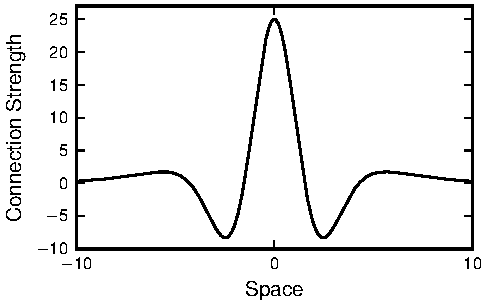
\includegraphics{./Graph/pdf/fig1.pdf} 
 % \end{center}
 % \caption{}
 % \label{fig:Figure1}
 % \end{figure*}

\item A few comments on how to adapt the smoother for real time implementation would be helpful. I presume that one would perform the smoothing during a training phase. But one would also wish to adapt in real time as observation or control scenarios progressed. A few words of perspective would be invaluable to help others translate the author's wisdom on this method to other applications.

\emph{A few comments have been added to the `Extensions to the Framework' section of the discussion.}

\item Figure 4. Should the axes be indicated as spatial frequency rather than just Hz?

\emph{Yes. Axes of Figure 4. (and also Figure 5.) are now changed to spatial frequency. The unit of the spatial frequency within the text is changed to cycles/mm.}

\item Page 45, Appendix D, Par 1, line 6: should `transform of a n-' should be `transform of an n-' ? I am grammatically challenged perhaps.

\emph{We stand corrected. We have changed the text to `an n-dimensional'.}

\end{enumerate}

\end{document}